\documentclass[tikz,border=10pt]{standalone}
\usepackage{tikz}
\usetikzlibrary{shapes,arrows,positioning,shadows,fit,calc}

\begin{document}

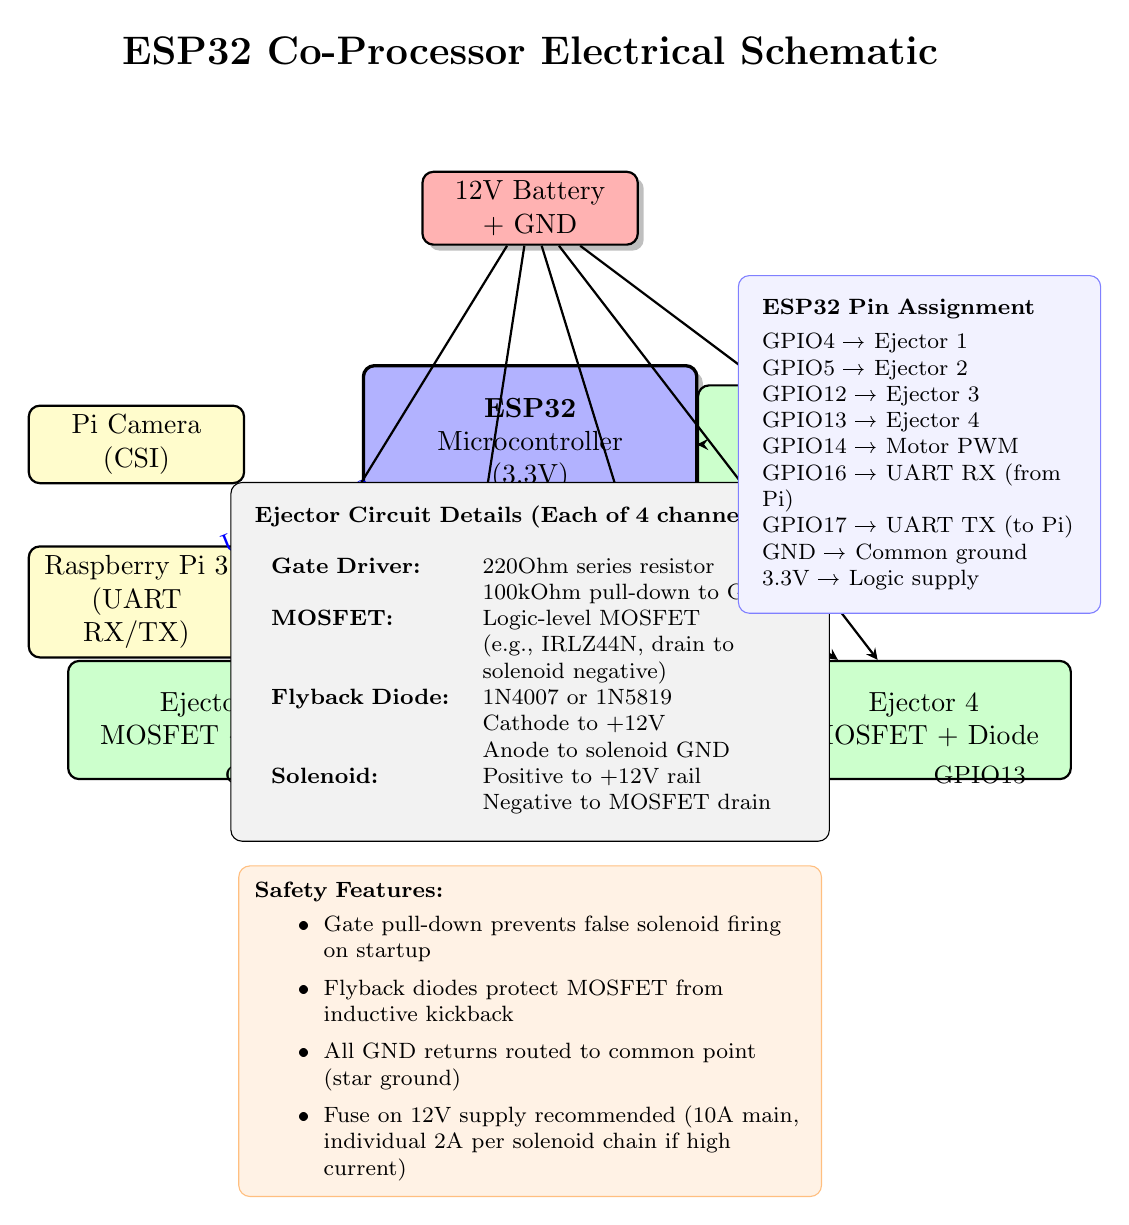
\begin{tikzpicture}[
    node distance=1.2cm,
    processor/.style={rectangle, draw, fill=blue!30, text width=4cm, text centered, rounded corners, minimum height=2cm, drop shadow, very thick},
    power/.style={rectangle, draw, fill=red!30, text width=2.5cm, text centered, rounded corners, minimum height=0.8cm, drop shadow, thick},
    circuit/.style={rectangle, draw, fill=green!20, text width=3.5cm, text centered, rounded corners, minimum height=1.5cm, thick},
    io/.style={rectangle, draw, fill=yellow!20, text width=2.5cm, text centered, rounded corners, minimum height=0.8cm, thick},
    arrow/.style={thick,->,>=stealth},
    label/.style={font=\small, anchor=west}
]

% Title
\node[font=\bfseries\Large] (title) at (0, 13) {ESP32 Co-Processor Electrical Schematic};

% Power supply
\node[power] (pwr) at (0, 11) {12V Battery\\+ GND};

% ESP32 Microcontroller
\node[processor] (esp32) at (0, 8) {\textbf{ESP32}\\Microcontroller\\(3.3V)};

% Camera (Pi side - reference only)
\node[io] (camera) at (-5, 8) {Pi Camera\\(CSI)};
\node[io] (pi) at (-5, 6) {Raspberry Pi 3\\(UART RX/TX)};

% UART connection
\draw[arrow, blue, very thick] (pi) -- node[above, sloped] {UART 115k2} (esp32);

% Vibrating Motor PWM
\node[circuit] (motor) at (4, 8) {Vibrating Motor\\PWM Control};
\node[label] at (4, 7.3) {GPIO14 → PWM};
\node[label] at (4, 6.9) {12V Motor Driver};
\draw[arrow] (esp32) -- (motor);
\draw[arrow] (pwr) -- (motor);

% Ejector circuits (4 total)
\node[circuit] (eject1) at (-4, 4.5) {Ejector 1\\MOSFET + Diode};
\node[label] at (-4, 3.8) {GPIO4};
\draw[arrow] (esp32) -- (eject1);
\draw[arrow] (pwr) -- (eject1);

\node[circuit] (eject2) at (-1, 4.5) {Ejector 2\\MOSFET + Diode};
\node[label] at (-1, 3.8) {GPIO5};
\draw[arrow] (esp32) -- (eject2);
\draw[arrow] (pwr) -- (eject2);

\node[circuit] (eject3) at (2, 4.5) {Ejector 3\\MOSFET + Diode};
\node[label] at (2, 3.8) {GPIO12};
\draw[arrow] (esp32) -- (eject3);
\draw[arrow] (pwr) -- (eject3);

\node[circuit] (eject4) at (5, 4.5) {Ejector 4\\MOSFET + Diode};
\node[label] at (5, 3.8) {GPIO13};
\draw[arrow] (esp32) -- (eject4);
\draw[arrow] (pwr) -- (eject4);

% Detailed ejector circuit (expanded view)
\node[below=3cm of pwr, text width=7cm, draw, fill=gray!10, rounded corners, inner sep=0.3cm, anchor=north, font=\footnotesize] (detail) {
    \textbf{Ejector Circuit Details (Each of 4 channels):}\\[0.2cm]
    \vspace{0.1cm}
    \begin{tabular}{ll}
        \textbf{Gate Driver:} & 220Ohm series resistor \\
        & 100kOhm pull-down to GND \\
        \textbf{MOSFET:} & Logic-level MOSFET \\
        & (e.g., IRLZ44N, drain to \\
        & solenoid negative) \\
        \textbf{Flyback Diode:} & 1N4007 or 1N5819 \\
        & Cathode to +12V \\
        & Anode to solenoid GND \\
        \textbf{Solenoid:} & Positive to +12V rail \\
        & Negative to MOSFET drain
    \end{tabular}
};

% Pin summary table
\node[right=0.5cm of esp32, text width=4cm, draw=blue!50, fill=blue!5, rounded corners, inner sep=0.3cm, anchor=west, font=\footnotesize] (pins) {
    \textbf{ESP32 Pin Assignment}\\[0.1cm]
    GPIO4 → Ejector 1\\
    GPIO5 → Ejector 2\\
    GPIO12 → Ejector 3\\
    GPIO13 → Ejector 4\\
    GPIO14 → Motor PWM\\
    GPIO16 → UART RX (from Pi)\\
    GPIO17 → UART TX (to Pi)\\
    GND → Common ground\\
    3.3V → Logic supply
};

% Safety notes
\node[below=0.3cm of detail, text width=7cm, draw=orange!50, fill=orange!10, rounded corners, inner sep=0.2cm, anchor=north, font=\footnotesize] (safety) {
    \textbf{Safety Features:}
    \begin{itemize}
        \item Gate pull-down prevents false solenoid firing on startup
        \item Flyback diodes protect MOSFET from inductive kickback
        \item All GND returns routed to common point (star ground)
        \item Fuse on 12V supply recommended (10A main, individual 2A per solenoid chain if high current)
    \end{itemize}
};

\end{tikzpicture}

\end{document}
